\documentclass[12pt]{article}
\usepackage{graphicx}
\usepackage{amssymb}
\usepackage{epstopdf}
\usepackage{amsmath}
\usepackage{multicol}
\usepackage{tcolorbox}
\usepackage{geometry}
\usepackage{enumitem}
\usepackage{fancyhdr}

\DeclareGraphicsRule{.tif}{png}{.png}{`convert #1 `dirname #1`/`basename #1 .tif`.png}

\textwidth = 6.5 in
\textheight = 9 in
\oddsidemargin = 0.0 in
\evensidemargin = 0.0 in
\topmargin = -23pt
\headheight = 0.0 in
\headsep = 0.0 in
\parskip = 0.2in
\parindent = 0.0in
\pagestyle{fancy}
\pagenumbering{gobble}

\newtheorem{theorem}{Theorem}
\newtheorem{corollary}[theorem]{Corollary}
\newtheorem{definition}{Definition}
%\includegraphics [height=50mm, width=50mm]{PathInt.jpg}
\title{Title} 

\begin{document}
%INSTRUCTOR NOTES
%No warm-up on quiz days. If wanted, today's warm-up would be solving equations.
 Name:
 \begin{center}\large{2.3 Derivative Function Preview}\end{center}

\begin{enumerate}
\item Match each of the functions on the left with their derivative functions on the right. Explain your reasoning.

\begin{center}
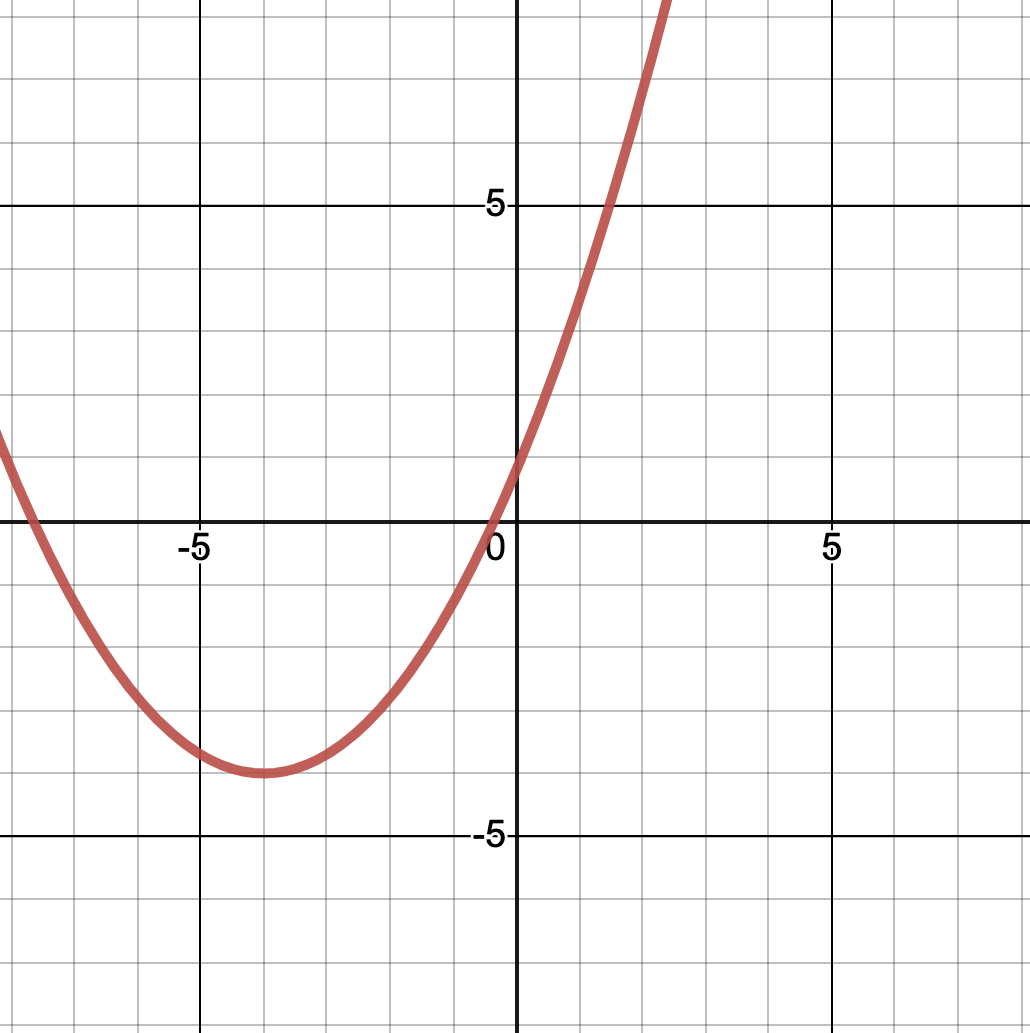
\includegraphics [height=89px]{r1} \hspace{50mm} 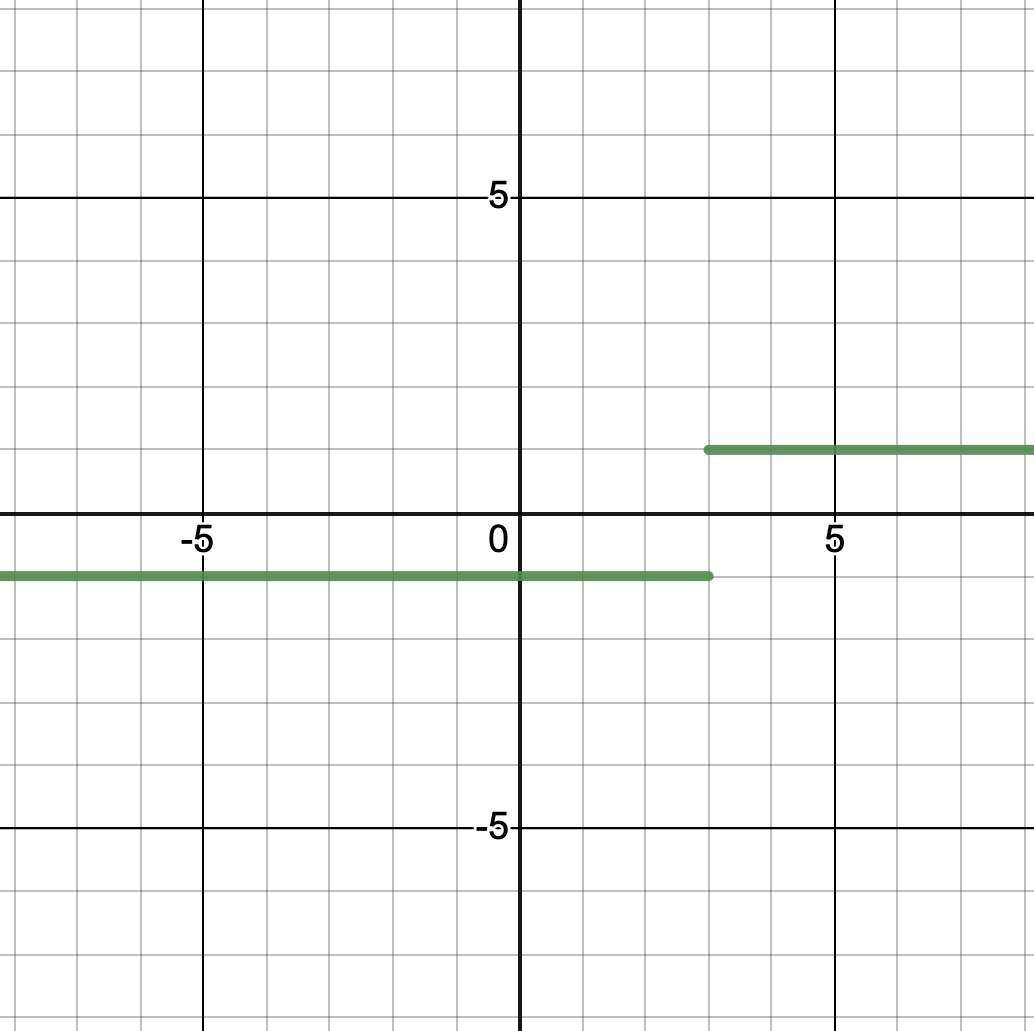
\includegraphics [height=89px]{g4}\\
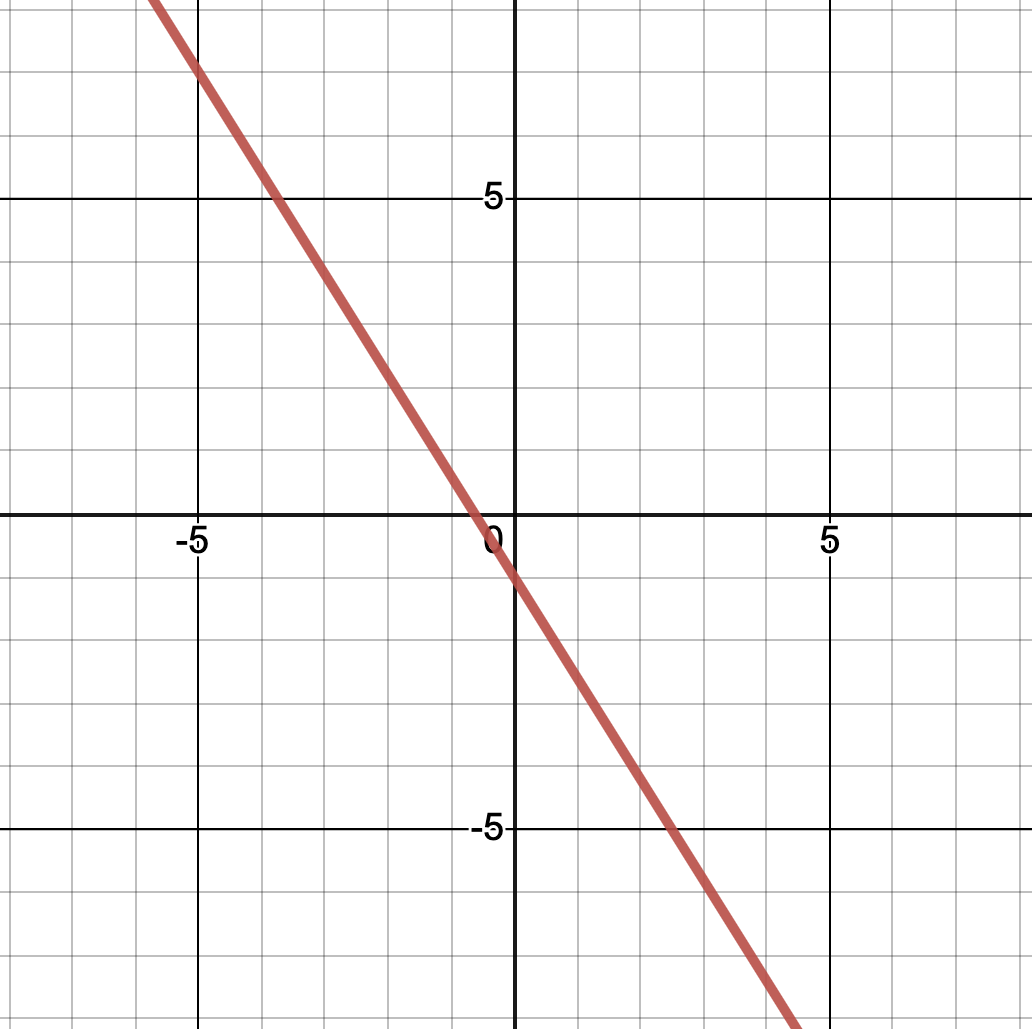
\includegraphics [height=89px]{r2} \hspace{50mm} 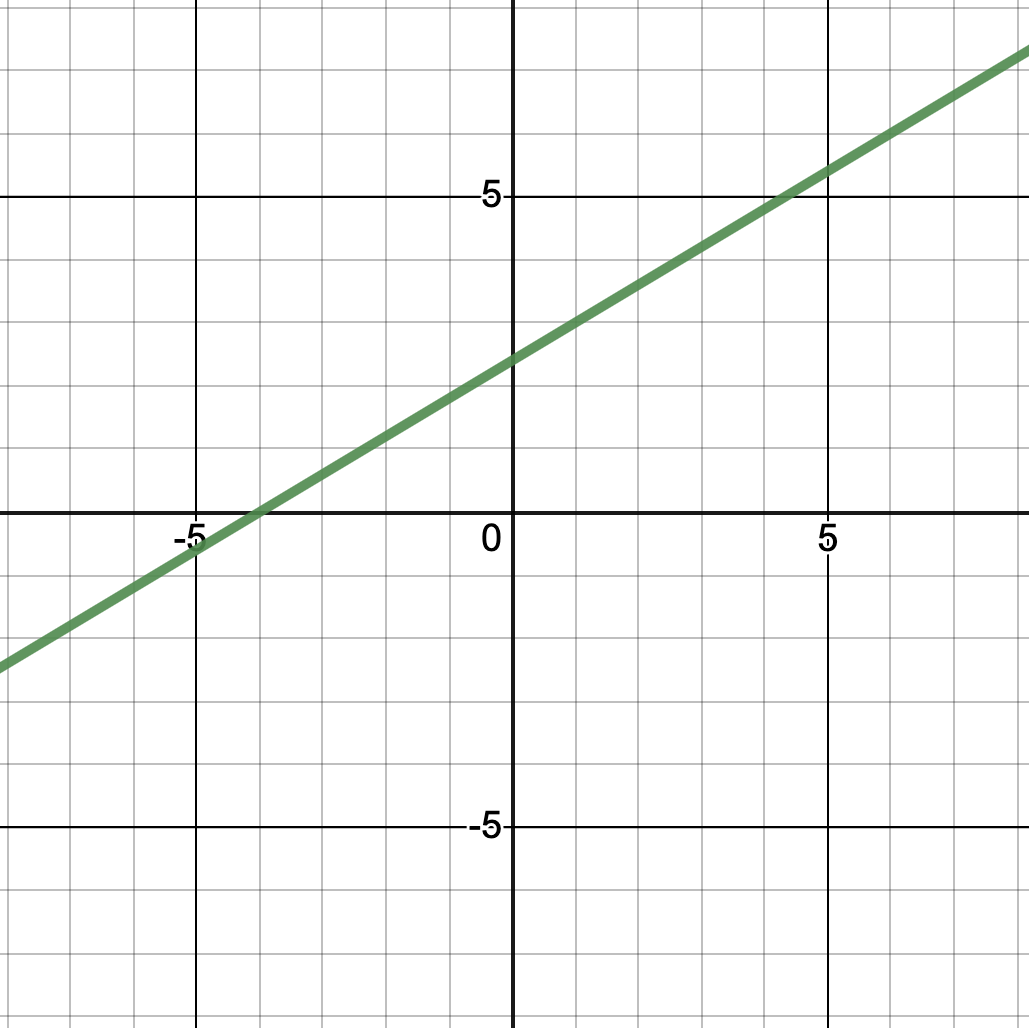
\includegraphics [height=89px]{g5}\\
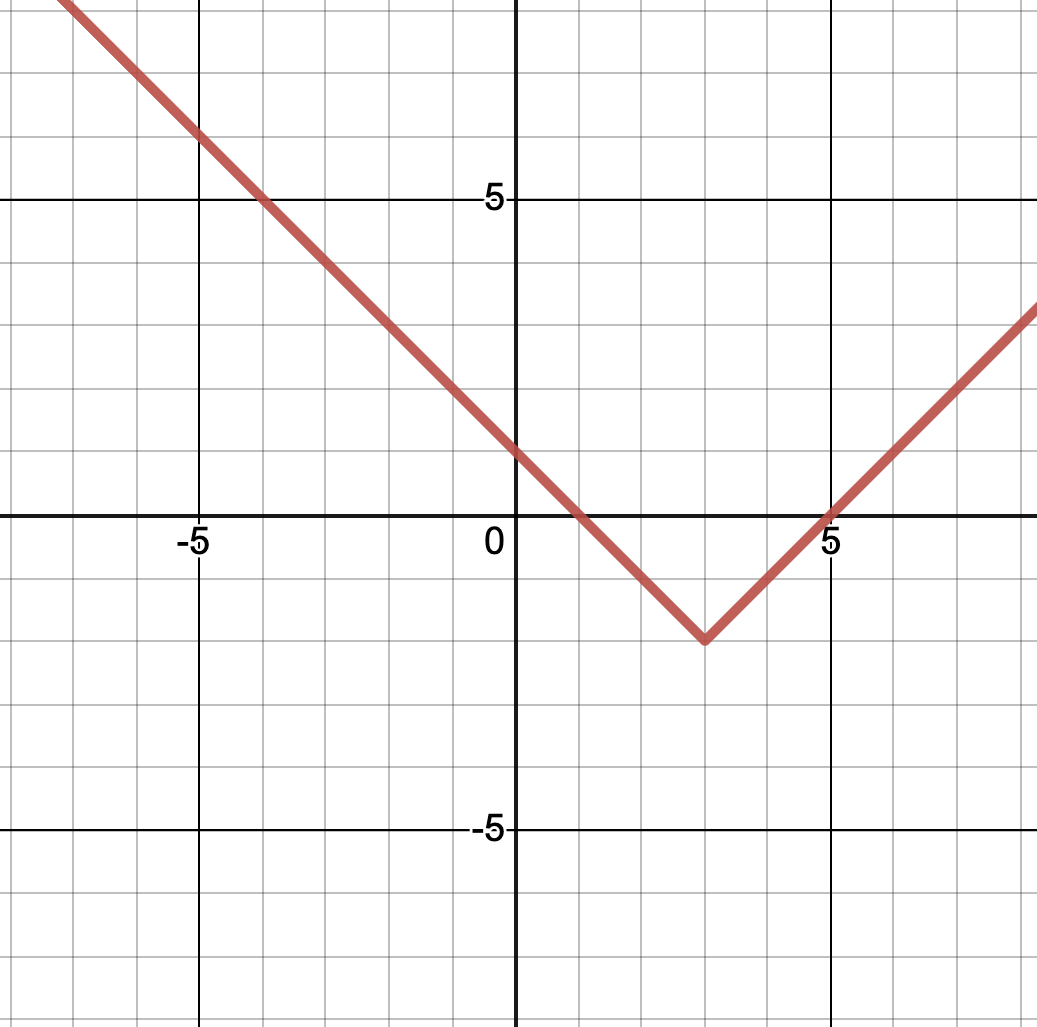
\includegraphics [height=89px]{r3} \hspace{50mm} 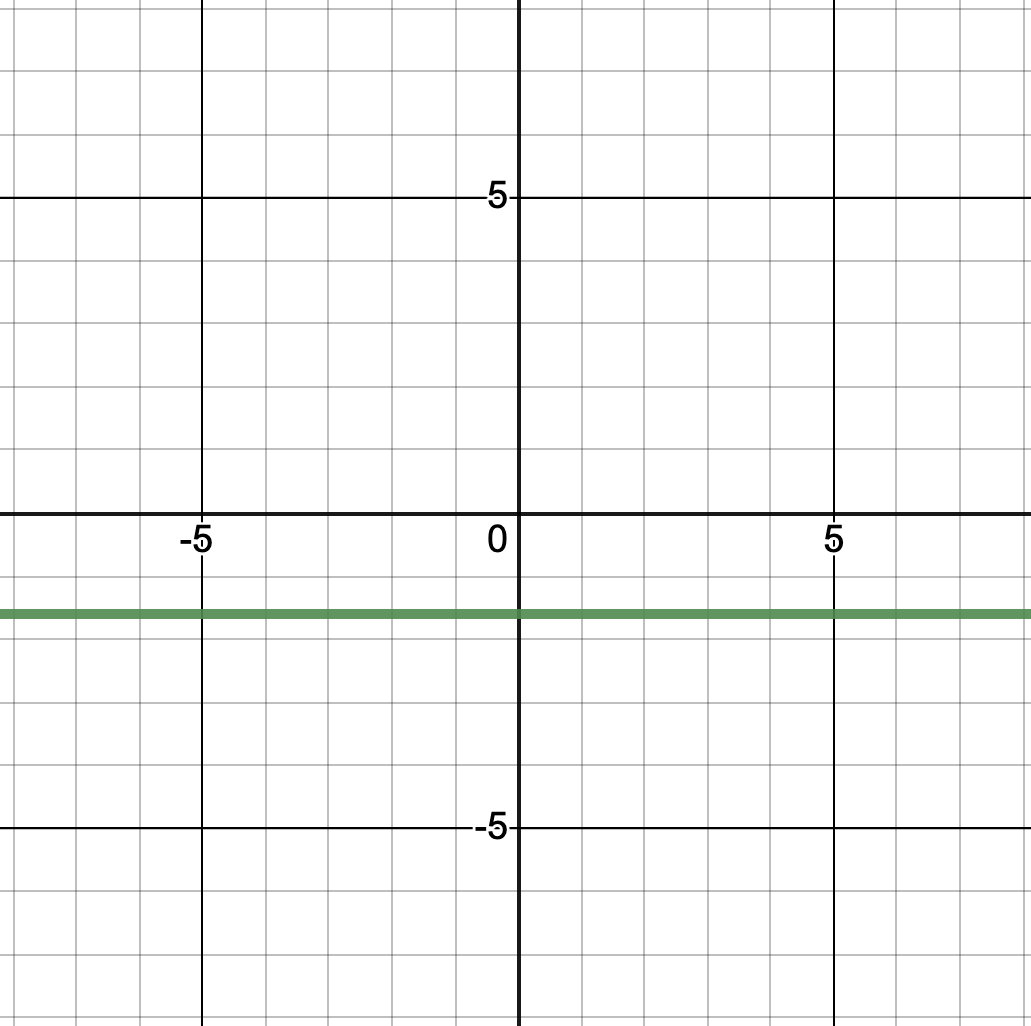
\includegraphics [height=89px]{g6}\\
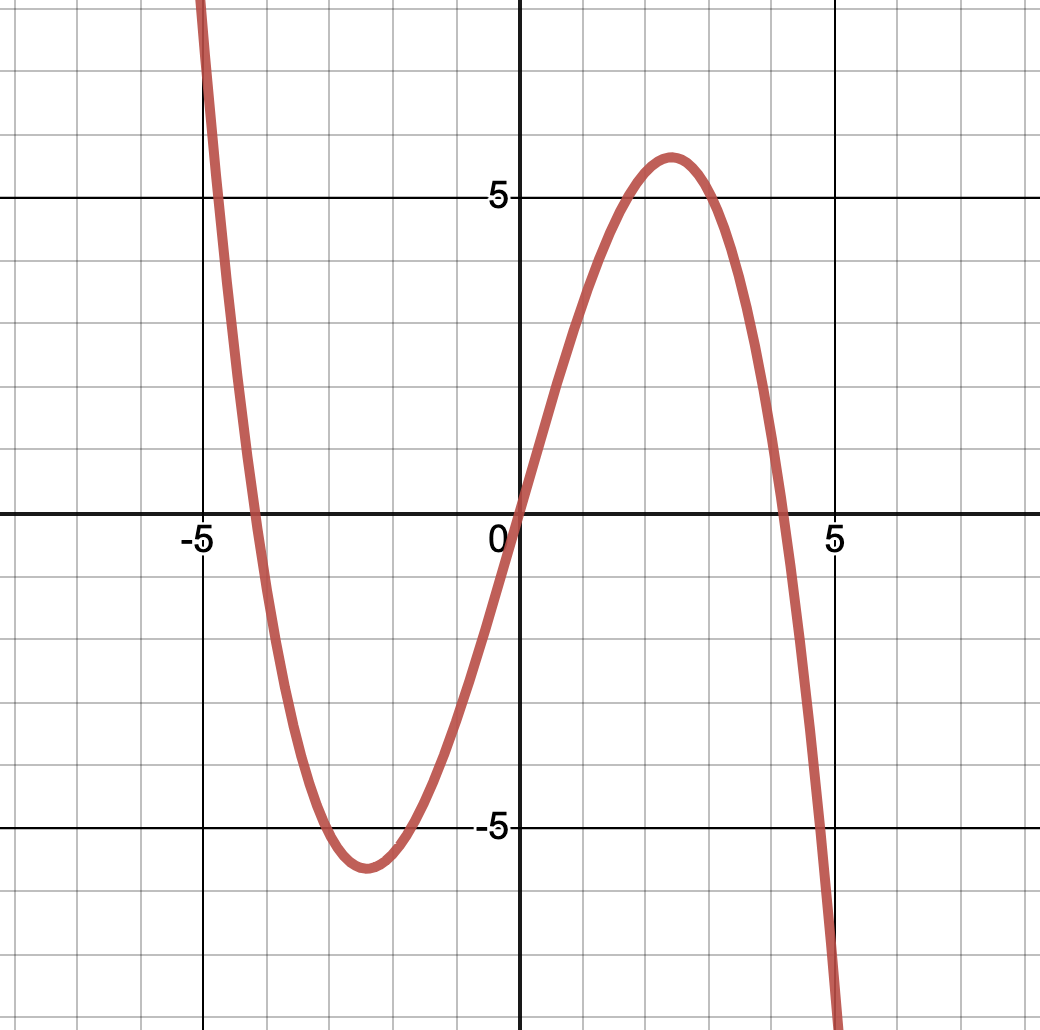
\includegraphics [height=89px]{r4} \hspace{50mm} 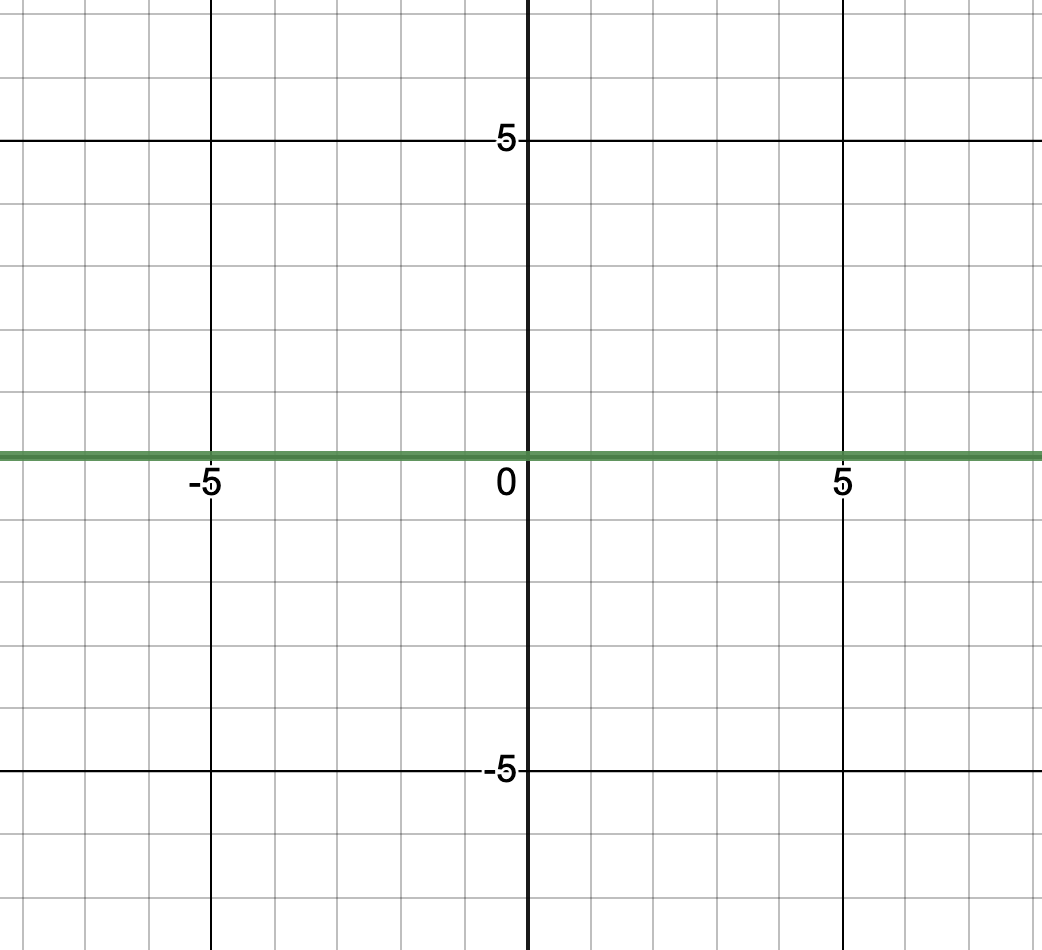
\includegraphics [height=89px]{g3}\\
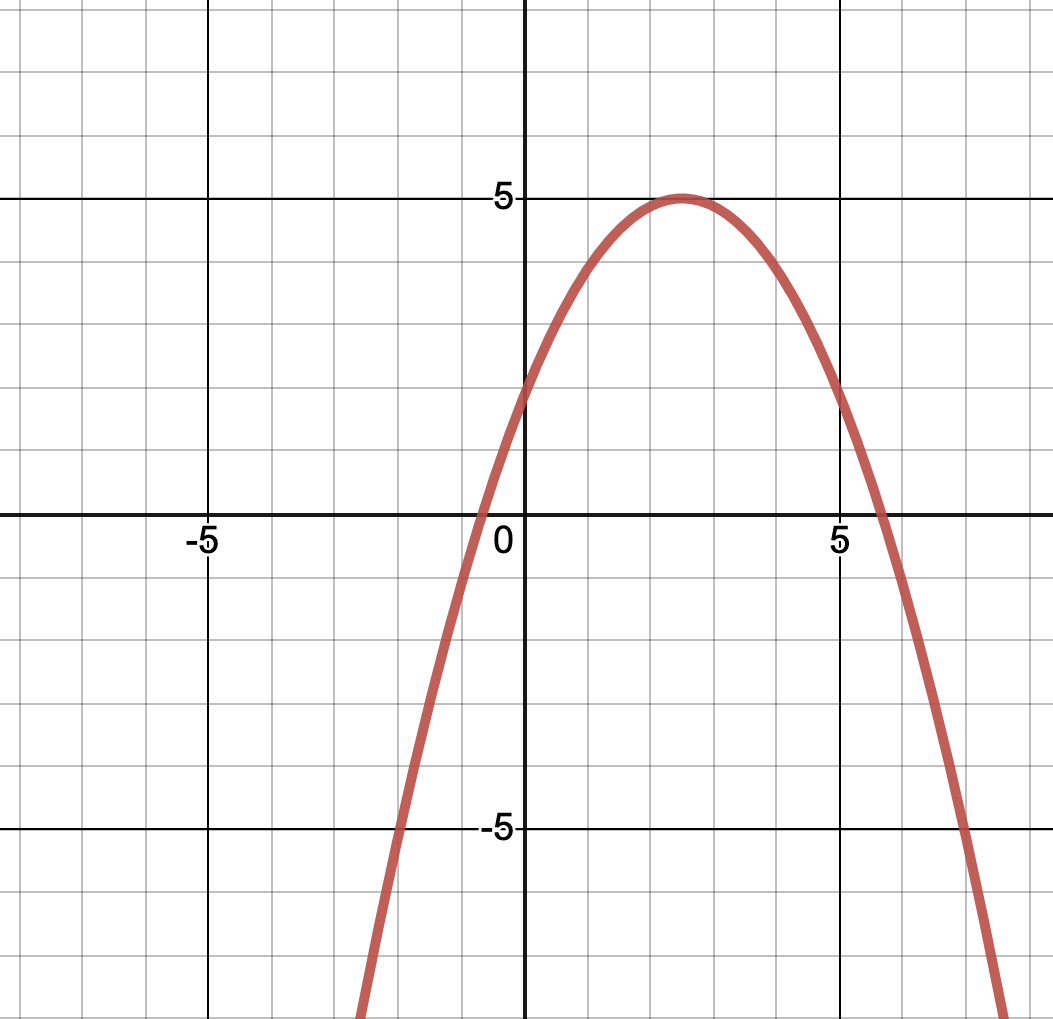
\includegraphics [height=89px]{r5} \hspace{50mm} 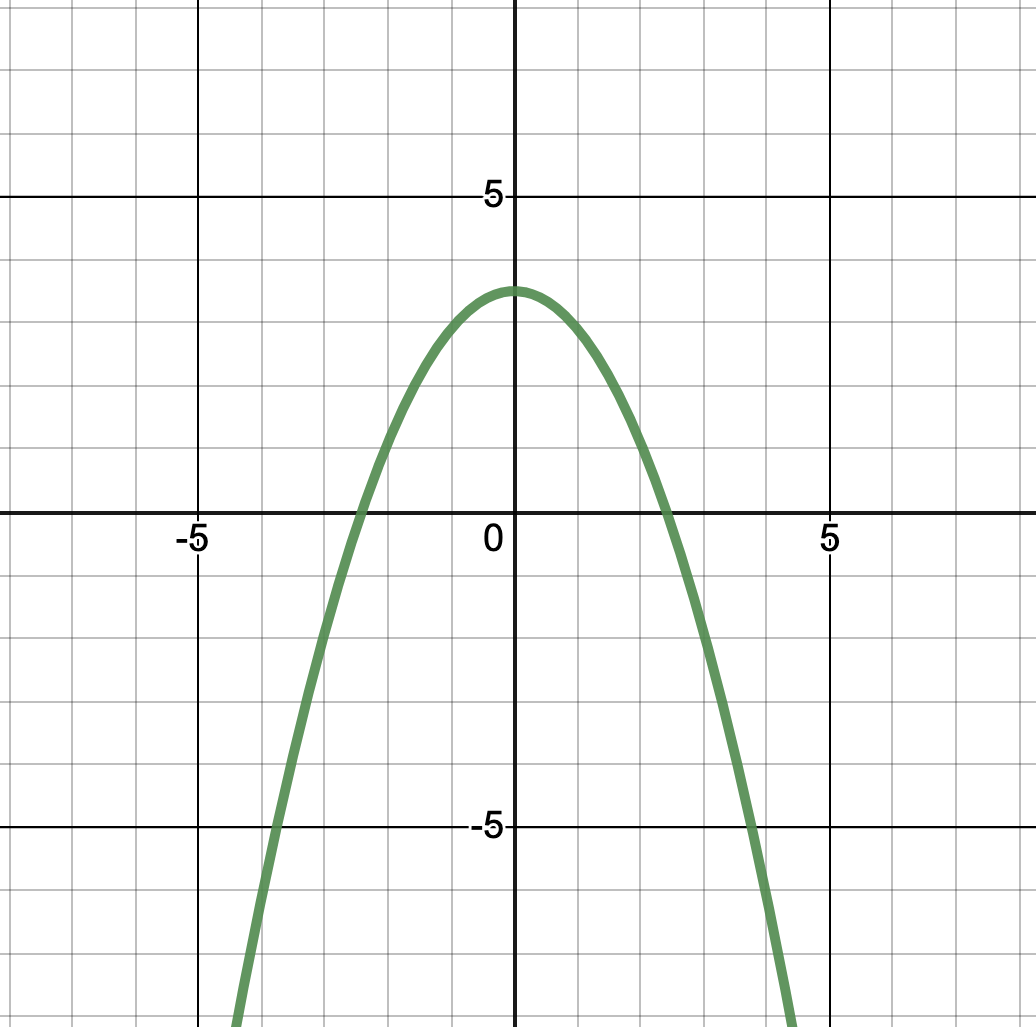
\includegraphics [height=89px]{g1}\\
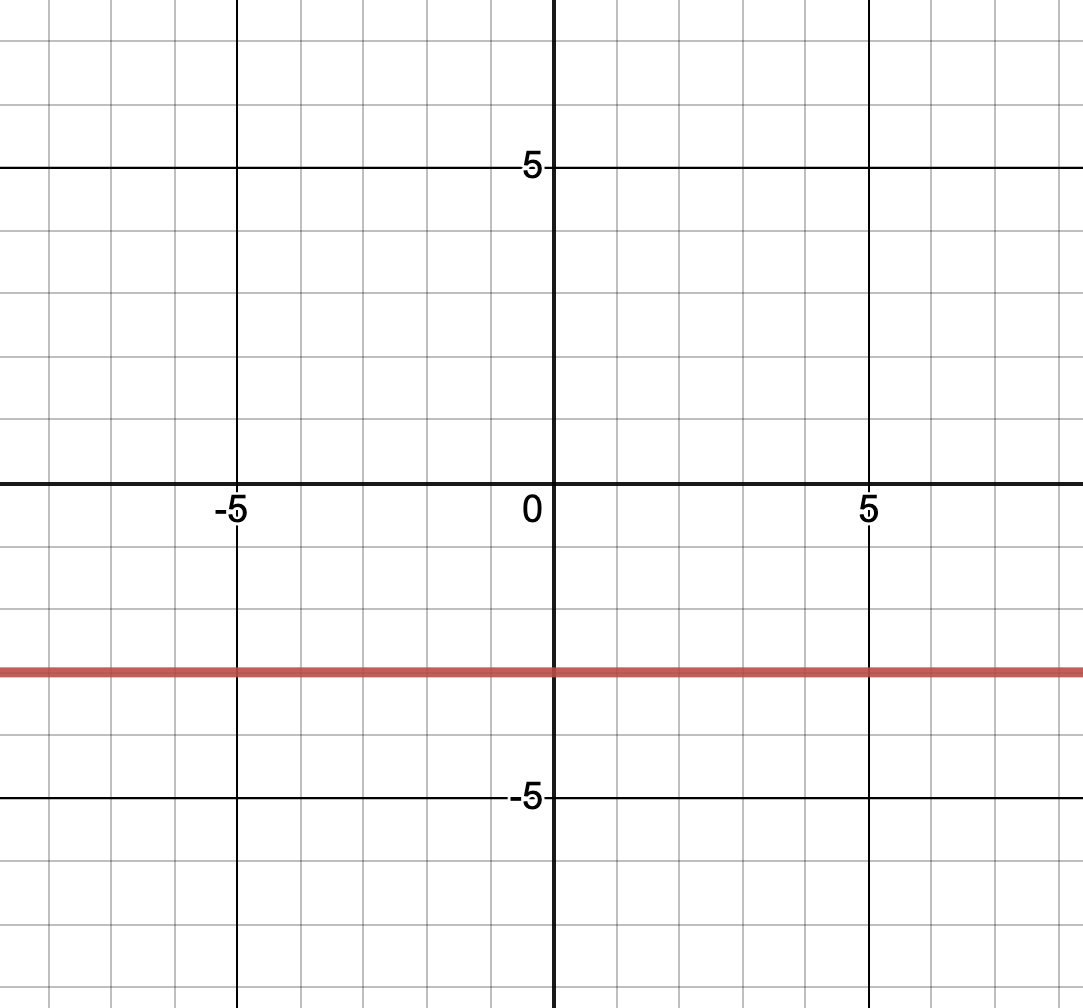
\includegraphics [height=89px]{r6} \hspace{50mm} 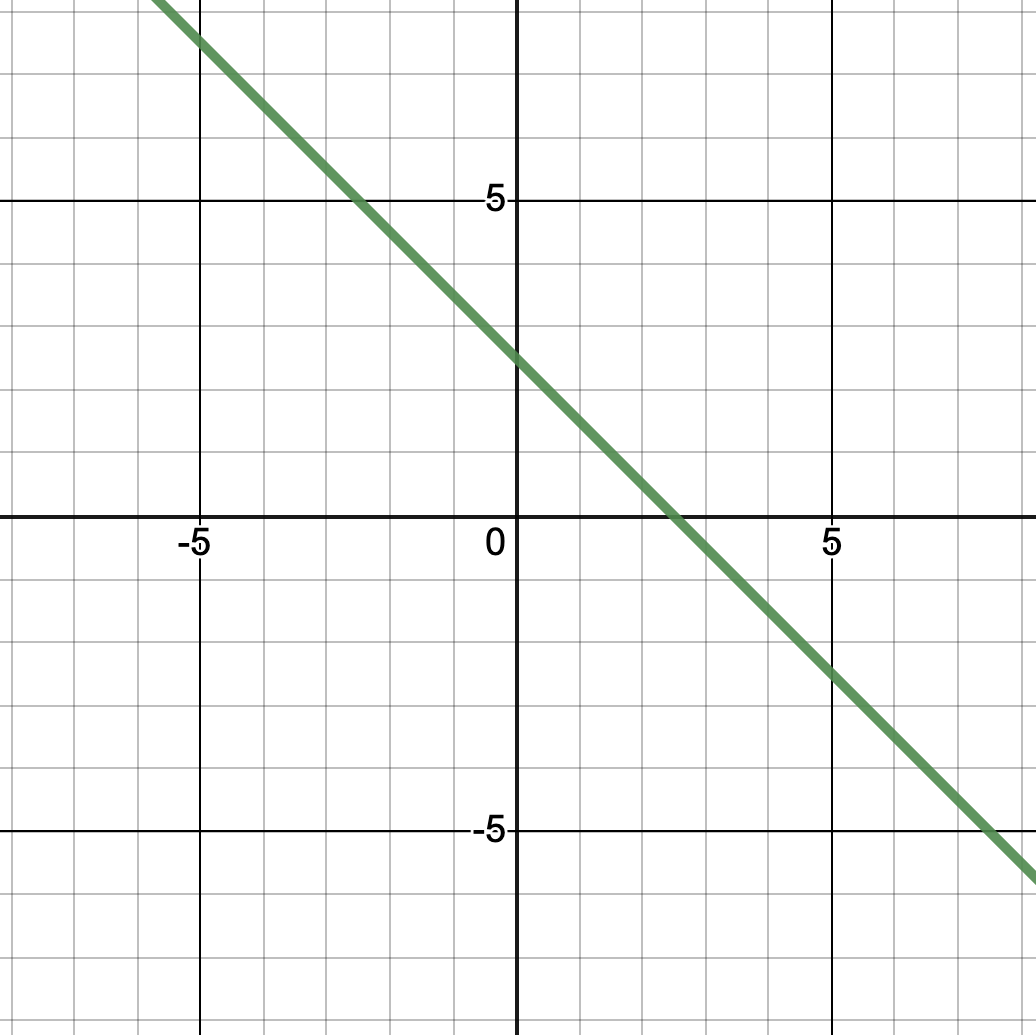
\includegraphics [height=89px]{g2}\\
\end{center}

\newpage

\hspace{10px}\\

\item Below you are given the graph of a function $f(x)$. With a straightedge, draw in tangent lines to $f(x)$ at every half unit and estimate their slope from the grid. Use your slopes to draw a graph of $f'(x)$ on the same set of axes.\\
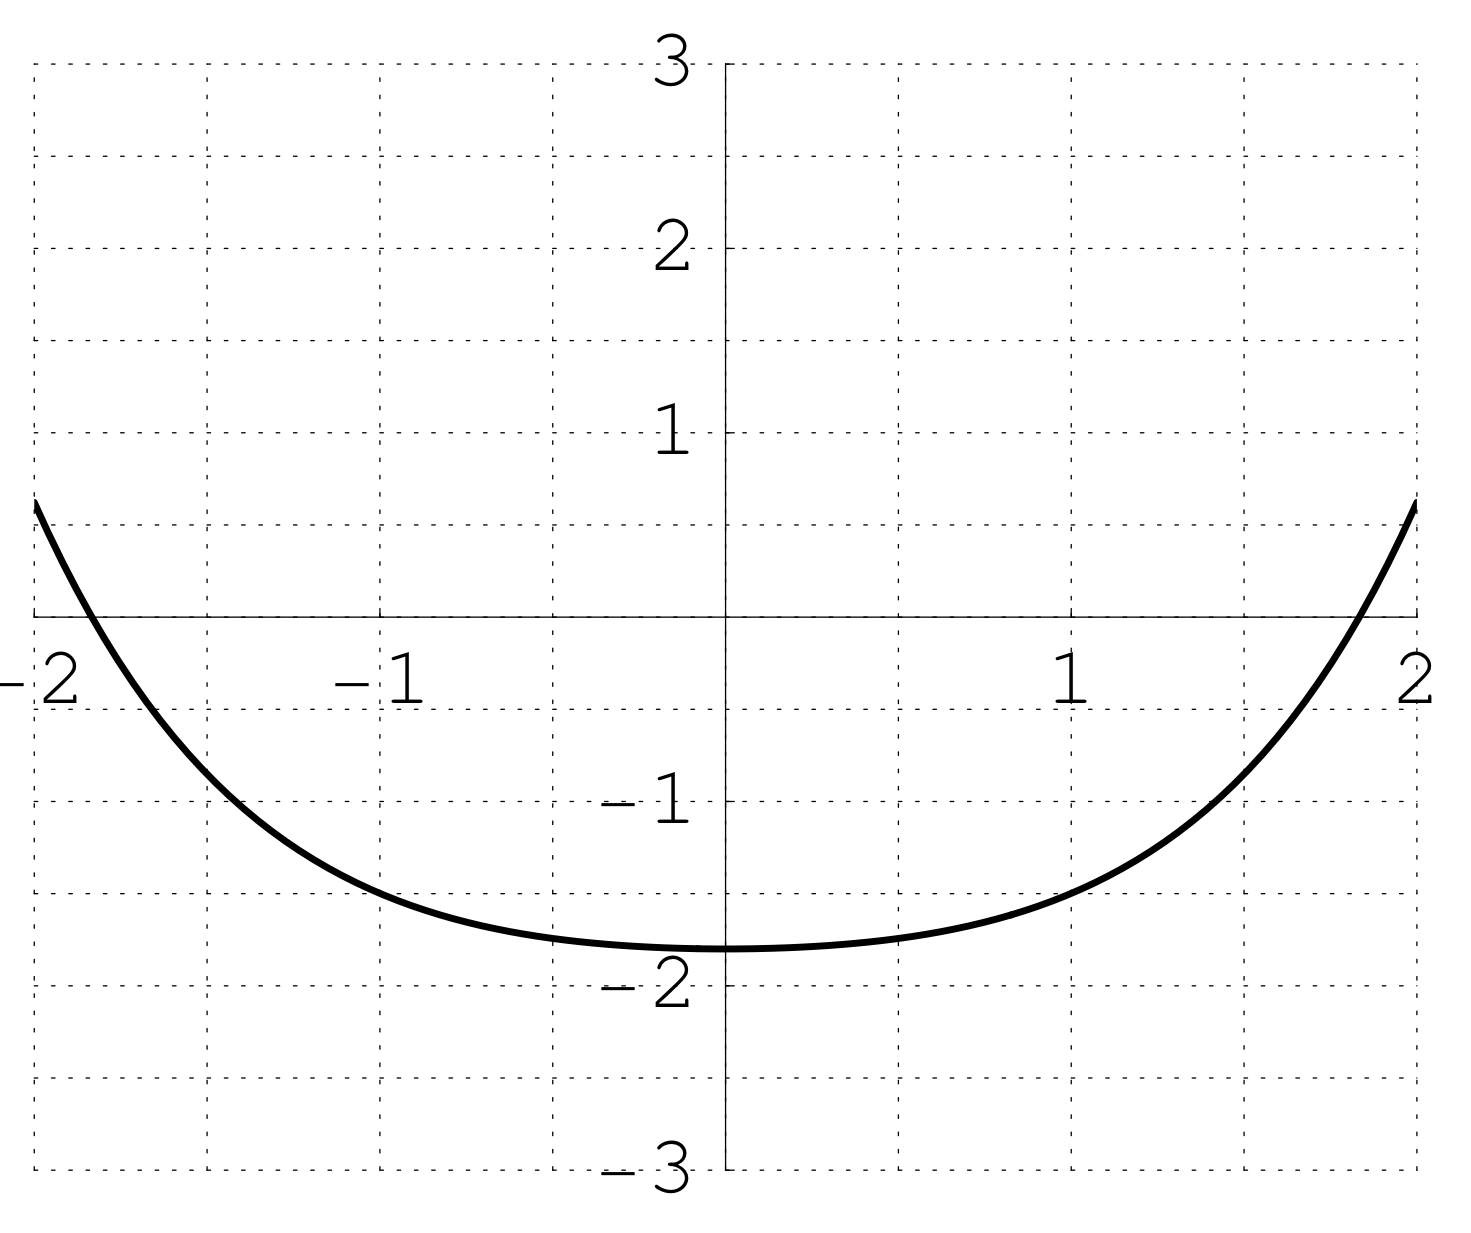
\includegraphics [height=50mm, width=70mm]{2_3_1}
\vfill

\item The graph below is the position of an ant over time, where positive positions are north of the ant colony, and negative positions are south of the ant colony. Sketch a rough graph of the velocity of the ant on the same axes.\\
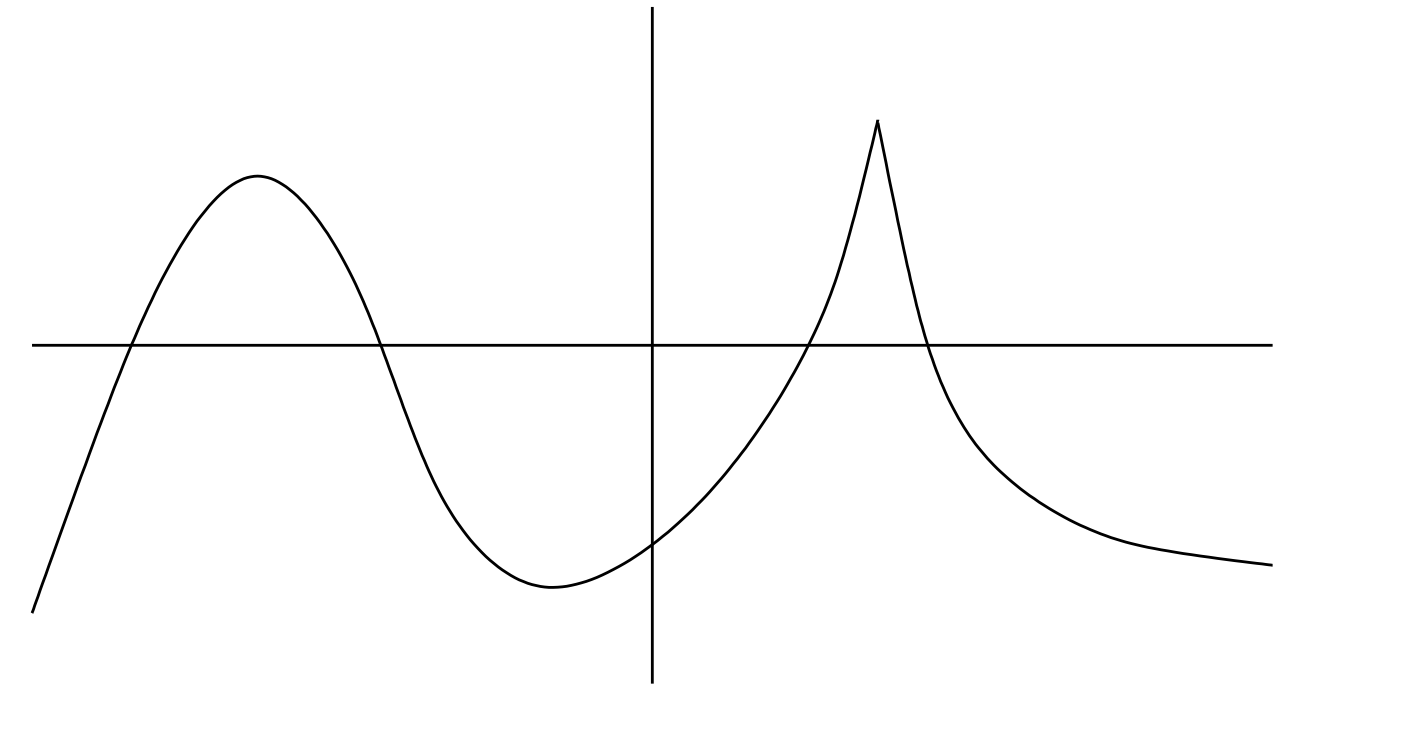
\includegraphics [height=50mm, width=70mm]{2_3_2}
\vfill

\item Given the graph of $f(x)$ below, sketch an accurate graph of $f'(x)$.\\
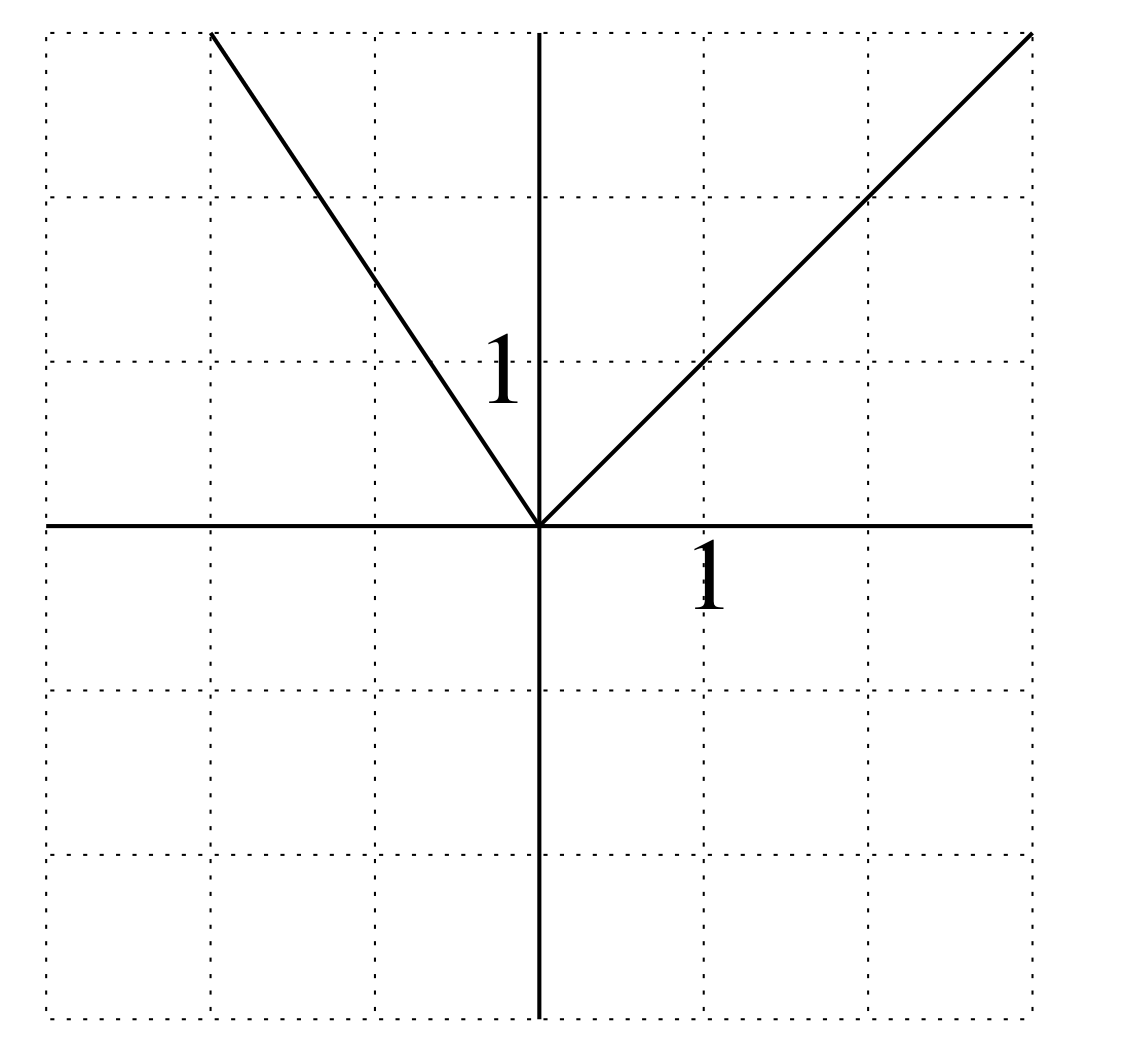
\includegraphics [height=50mm, width=70mm]{2_3_3}
\vfill

\end{enumerate}
\end{document} 